\newsection
\subsection{Robustness to distribution shifts} 
\label{sec:robustness}
\sectionauthors{Sang Michael Xie, Ananya Kumar, Rohan Taori, Tony Lee, Shiori Sagawa, Pang Wei Koh, Tatsunori Hashimoto}

Real-world ML systems need to be robust to distribution shifts\dash{}they should work well on test distributions which differ from the train distribution.
High-stakes applications such as poverty mapping in under-resourced countries~\citep{xie2016transfer,jean2016combining}, self-driving cars~\citep{yu2020bdd100k,sun2020scalability}, and medical diagnosis~\citep{ albadawy2018tumor,dai2018dark} all require models that generalize well to circumstances not seen in the training data,
\eg test examples from different countries, under different driving conditions, or from different hospitals.
Prior work has shown that these types of distribution shifts can cause large drops in performance even in state-of-the-art models~\citep{blitzer2006domain,daume07easyadapt,sugiyama2007covariate,ganin2015domain,peng2019moment,kumar2020gradual,arjovsky2019invariant,szegedy2014intriguing,hendrycks2019benchmarking,sagawa2020group,recht2019doimagenet,abney2007semisup,ruder2018strong,geirhos2018generalisation,kumar2020conservative,yu2020mopo,geirhos2020shortcut,xie2021innout,koh2021wilds}. 

\newcommand\ppre{p_{\text{pre}}}
\newcommand\ptrain{p^{\sT}_{\text{ID}}}
\newcommand\ptest{p^{\sT}_{\text{OOD}}}


In this section, we consider the role of foundation models on robustness to distribution shifts. A foundation model is trained on a large and diverse unlabeled dataset sampled from a distribution $\ppre$ and can be adapted to many downstream tasks.
For each downstream task $\sT$, the foundation model is adapted to labeled training data sampled from an in-distribution (ID) training distribution $\ptrain$, and then evaluated on an out-of-distribution (OOD) test distribution $\ptest$.
For example, a poverty prediction model~\citep{xie2016transfer,jean2016combining} may be pretrained on unlabeled satellite data from across the world to learn useful features for all countries, then fine-tuned on labeled examples from Nigeria, and finally evaluated in Malawi where labeled examples are scarce.

We argue that 1) foundation models are a particularly promising approach to robustness. Existing work shows that pretraining on unlabeled data is an effective, general-purpose way to improve accuracy on OOD test distributions, in contrast to many robustness interventions which are constrained to narrow types of distribution shifts. However, we also discuss why 2) foundation models may not always mitigate distribution shifts, such as certain shifts due to spurious correlations or changes over time. Finally, 3) we outline several research directions to leverage and improve foundation models for robustness.

We note that one of the ways in which foundation models lead to improved extrapolation is by providing inductive biases (via model initialization) for the adapted model, which are learned on a diverse dataset that extends beyond the downstream training data. However, this same inductive bias can also encode harmful associations from the pretrained data and lead to representational and allocational harms in the presence of distribution shift. See \refsec{data} and \refsec{fairness} for further discussion of such harms and methods for mitigation.


\begin{figure}[t]
\centering
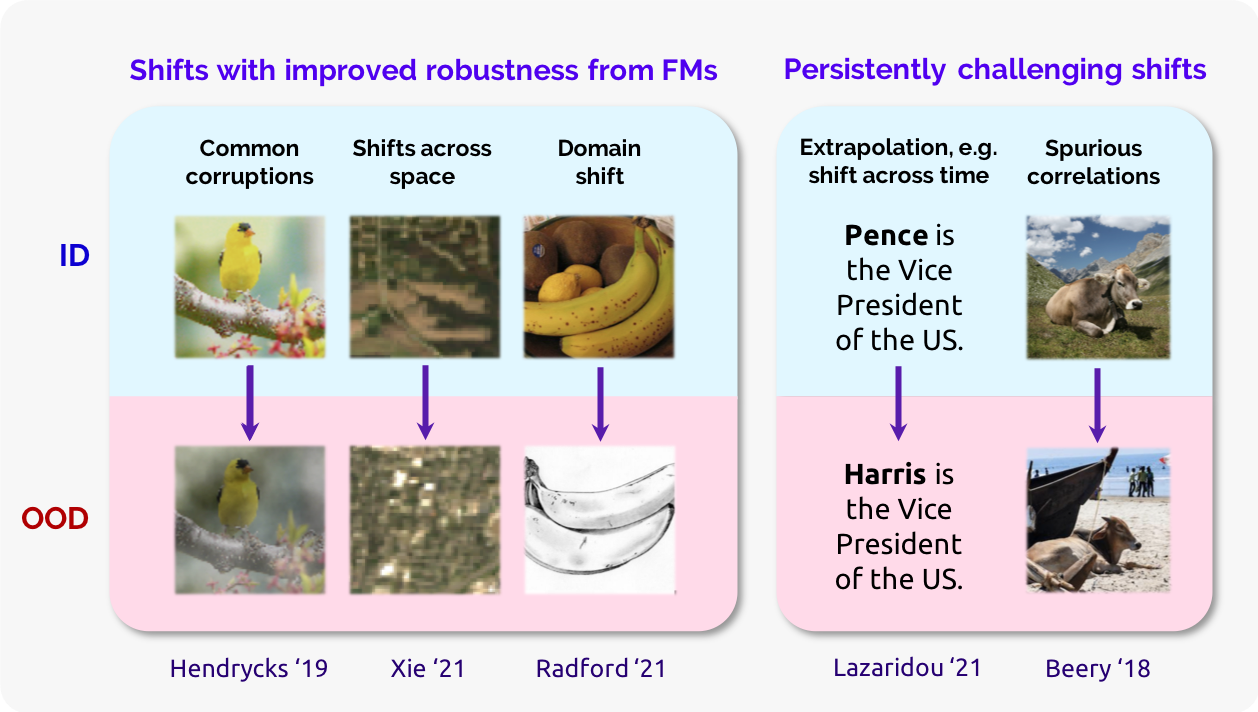
\includegraphics[width=0.85\linewidth]{technology/figures/Robustness.png}
\caption{\label{fig:robustness}  In-distribution (ID) and out-of-distribution (OOD) inputs for a variety of distribution shifts. We take the implied task to be image classification for images and fact verification for text.  Although representations learned by foundation models improve downstream robustness for many shifts (\eg common corruptions)~\citep{hendrycks2019benchmarking,xie2021innout,radford2021learning}, some shifts such as spurious correlations (where grass is predictive of cow)~\citep{beery2020iwildcam} and extrapolation across time (with facts that change over time)~\citep{lazaridou2021pitfalls} are still likely unaddressed by foundation models.
}
\end{figure}

\subsubsection{Advantages}
\label{sec:robustness-advantages}

By learning representations on a large and diverse foundation model training distribution $\ppre$, foundation models can improve accuracy of the adapted derivative on the downstream test distribution $\ptest$.
OpenAI's CLIP model, which is a foundation model trained on a diverse set of images and natural language, has been shown to be robust to a class of distribution shifts on ImageNet~\citep{radford2021learning}: 
for example, both CLIP and a standard ResNet50 obtain 76\% accuracy on ImageNet, but CLIP achieves 6\% higher accuracy on ImageNetV2 \citep{recht2019doimagenet} and 35\% higher accuracy on ImageNet Sketch~\citep{radford2021learning}, which are both related but different from the original ImageNet training distribution.
In contrast, many other robustness interventions, such as adversarial training~\citep{madry2018towards}, invariant risk minimization~\citep{arjovsky2019invariant}, or using larger models have had little impact on effective robustness (defined as the gap between in-distribution and out-of-distribution performance) on these ImageNet tasks, especially without explicit knowledge of the distribution shift \citep{taori2020measuring,santurkar2020breeds,radford2021learning,miller2021line}.

Many other works demonstrate that pretraining on large datasets can improve robustness to common image corruptions, label shift, and label corruptions \citep{hendrycks2019pretraining,hendrycks2019selfsupervised};  to natural geographic shifts in satellite imagery tasks~\citep{xie2021innout}; and to shifts across topics in natural language understanding tasks \citep{hendrycks2020pretrained,fisch2019mrqa,yogatama2019learning}.
As another example, diversifying the foundation model training data to multiple languages (as in multilingual BERT~\citep{liu2020multilingual}) significantly improves performance in unseen language pairs.


\subsubsection{Persistent challenges}
\label{sec:robustness-challenges}

Despite promising signs that foundation models will result in substantial improvements to robustness, we anticipate that foundation models are not a panacea for distribution shifts. We discuss this in the context of two broad categories of distribution shifts below.

\paragraph{Spurious correlations.} 
Spurious correlations are statistical correlations between features and labels with predictive power on the training distribution but not on a test distribution~\citep{heinze2017conditional, arjovsky2019invariant, sagawa2020group}.
Well-known examples include reliance on background color for object recognition~\citep{xiao2020noise}, surgical markers for medical diagnostics~\citep{winkler2019derm}, annotator biases in crowdsourced data~\citep{tsuchiya2018performance,gururangan2018annotation,poliak2018hypothesis,geva-etal-2019-modeling}, and demographic biases \citep{abid2021,stereoset,gehman-etal-2020-realtoxicityprompts}. 
Models learn these spurious correlations largely because the foundation model training and adaptation data exhibit these biases~\citep{nagarajan2020understanding,gehman-etal-2020-realtoxicityprompts}, and this issue cannot simply be addressed with larger models~\citep{sagawa2020overparameterization}.

Foundation models may exacerbate or mitigate the effects of spurious correlations, but this depends on the nature of the particular downstream task and its relation to the foundation model training data and algorithm. By training with a diverse dataset, foundation models may improve robustness to spurious correlations that are found only in a subset of the training data: \eg existing studies find that pretrained language models can avoid spurious correlations by quickly learning from counterexamples to the spurious correlations~\citep{tu2020empirical}.
However, foundation models can also exacerbate the issue by introducing biases present in the foundation model training data, as observed for demographic biases in GPT-3 and other NLP models~\citep{abid2021,stereoset,gehman-etal-2020-realtoxicityprompts}.
Moreover, training at scale alone need not fully address the root issue of identifying and not relying on the features that are predictive on the downstream training set but not on the downstream test set~\citep{heinze2017conditional}.
Addressing these challenges will require us to understand and manage the inductive bias from foundation model training and develop adaptation algorithms that are resistant to learning spurious correlations.

\paragraph{Extrapolation and temporal drift.} 

Finally, the few- and zero-shot capabilities of foundation models will mean that these models will increasingly be used far beyond the training distribution. While large-scale foundation model training can help with certain forms of extrapolation to new distributions ~\citep{papadimitriou2020learning}, there may be limits to their extrapolation capabilities. 
For example, existing language models cannot handle changes to world knowledge or language change without re-training~\citep{lazaridou2021pitfalls,dhingra2021time}, zero-shot transfer in CLIP suffers greatly in satellite image domains~\citep{radford2021learning}, and ImageNet pretraining does not substantially improve the performance of large models on medical images~\citep{raghu2019transfusion,ke2021chextransfer}.
We believe that foundation models cannot be assumed to automatically extrapolate within a given modality (\eg all images), and it will become increasingly important to define and separate the forms of extrapolation that are newly enabled by foundation models from those that remain out of reach.
Though existing taxonomies for distribution shifts have been proposed in generality~\citep{candela2009when,ye2021oodbench},
fully understanding and defining the types of distribution shifts for which foundation models are effective is a major open problem for robustness research.

\subsubsection{Opportunities}
\label{sec:robustness-opportunities}

Foundation models hold substantial promise as a general-purpose robustness intervention for distribution shifts, and open new avenues for robustness research. We outline some opportunities and open questions below.

\paragraph{Understanding foundation model representations.}
Existing studies of the robustness of foundation models have been largely empirical, and there is little understanding of the mechanism behind gains in robustness.
~\citet{sun2019unsupervised} hypothesize that pretrained representations
bring disparate domains (such as ID and OOD distributions) closer together, which can in turn improve generalization from labeled ID data to OOD data~\citep{ben2010theory}. Controlled experimentation on measuring the distance between domain representations with and without pretraining can elucidate this effect. There are initial promising directions in characterizing foundation model training (\eg contrastive learning as a spectral graph decomposition~\citep{haochen2021spectral}) and their inductive biases~\citep{SaMa20mat,lee2020predicting,zhang20ont,xie2020selftraining}.
However these theories are limited and fail to address other empirically effective foundation models such as fully generative language models (\eg GPT-3~\citep{brown2020gpt3} and image-GPT~\citep{chen2020imagegpt}). Further understanding how these inductive biases are useful under distribution shift may lead to a more complete theory (\refsec{theory}) of how foundation models improve robustness. 

\paragraph{Data augmentation in foundation model training.} 
While foundation models trained without knowledge of the downstream tasks can avoid some task-specific biases and often improve robustness, certain statistical biases stemming from how the foundation model was trained may persist.
As a concrete example, many contemporary self-supervision algorithms are heavily dependent on choosing an appropriate set of data augmentations \citep{chen2020simclr}, which in turn confers different types of robustness in the adaptation phase: \citet{xiao2021contrastive} show that a foundation model for vision trained with contrastive learning on rotation augmentations may improve OOD performance on adaptation tasks with rotation invariance, but may not improve robustness for tasks where OOD generalization requires other invariances.
Further research into what types of data augmentations improve robustness for a wide range of downstream tasks\dash{}including data augmentations that are learned from data \citep{wong2020learningpert,Tamkin2021ViewmakerNL} or designed to be generally applicable across data modalities \citep{verma2021towards}\dash{}will inform better foundation model training algorithms (\refsec{training}).

\paragraph{Encoding structure in foundation model training.}
In general, exploring new ways of encoding known structure and invariances in the data is an important path forward for foundation model training. Many real-world tasks have additional metadata (\eg spatial location coordinates, climate information from auxiliary satellites in poverty prediction), which may provide additional structure for OOD generalization (\eg across geographic areas)~\citep{xie2021innout,koh2021wilds}. For example,~\citet{xie2021innout} show that metadata can be used as targets for pretraining to improve downstream OOD accuracy. In language, modeling the tags in HTML data provides additional downstream-task-adjacent supervision, allows for new forms of prompting (\eg filling in \texttt{<title>} tags for title suggestion), and improves data efficiency~\citep{aghajanyan2021HTLM}. While current data augmentation methods encode hand-crafted knowledge, other avenues such as exploiting metadata could provide a more automated way of determining which structures and invariances to incorporate for foundation model training. 

\paragraph{Specialization vs.~diversity in foundation model training data.}
The choice of foundation model training data has downstream effects\dash{}training on a more diverse dataset is not always better for downstream performance than a more specialized foundation model~\citep{cole2021contrastive,chalkidis2020legal} (see \refsec{adaptation} for a more detailed discussion).
In some domains such as satellite images and specialized text topics, continued pretraining on the specialized domain improves the downstream performance significantly~\citep{reed2021selfsupervised,gururangan2020dont}.
This is a potential source of tension: on one hand, we might want to train the foundation model on a large, diverse dataset in order to have more robust performance under distribution shifts, while on the other hand, we might need to specialize the foundation model to improve its in-distribution and out-of-distribution performance on downstream tasks.
A better understanding of how specialization affects the in-distribution and out-of-distribution performance of foundation models will allow us to design and collect more effective foundation model training sets.

\paragraph{Adaptation methods.}
Although foundation models provide a strong starting point, how the adaptation method uses the pretrained information can affect robustness.
For instance, lightweight tuning methods for language models (\eg adapter/prefix/prompt tuning~\citep{houlsby19adapter,li2021prefix,lester2021power}), which adapt the model for a new task by optimizing a small set of parameters (such as a continuous prompt) while keeping the other foundation model parameters frozen, seem to give OOD performance benefits (\refsec{adaptation}).
~\citet{xie2021composed} explain this in a special case, where composing a learned model with a frozen foundation model can reduce the complexity of the learned model, improving generalization both ID and OOD. However, it is poorly understood in general why freezing parameters seems to improve OOD performance.
Finally, while current adaptation methods may suffice for good ID generalization, they do not explicitly account for distribution shift. As a first step, we can investigate how methods for distribution shifts such as domain adaptation, domain generalization, and semi-supervised learning methods interact with foundation models when used for adaptation. Progress in these directions can lead to adaptation methods that can better leverage foundation models for robustness.